\documentclass{beamer}
\usepackage{beamerthemeshadow}
\usepackage{graphicx}
\usepackage{color}
\usepackage[utf8]{inputenc}
\usepackage{hyperref}
\usepackage[flushleft]{threeparttable}
\usepackage[serbian]{babel}
\usetheme{Warsaw}
\definecolor{beamer@pearlyPurple}{rgb}{0.71,0.4,0.63}
\setbeamercolor{structure}{fg=beamer@pearlyPurple}

\def\d{{\fontencoding{T1}\selectfont\dj}}
\def\D{{\fontencoding{T1}\selectfont\DJ}}


\title{AI koji generiše sliku na osnovu teksta}
\author{Budimir Nikola\\ Trajković Miljan\\ Cvejić Miloš\\ Bajić Bogdan}
\institute{Matematički fakultet\\Univerzitet u Beogradu}
\date{
	\footnotesize{Beograd, 2022.}	
}

\begin{document}
\begin{frame}
	\thispagestyle{empty}
	\titlepage
\end{frame}

\addtocounter{framenumber}{-1}

\begin{frame}[fragile]\frametitle{Literatura}
	\begin{itemize}
		\item \url{https://www.cse.unsw.edu.au/ cs9417ml/RL1/introduction.html}\\
		\item Stanislav Frolov, Tobias Hinz, Federico Raue, Jörn Hees, Andreas Den-
gel, Adversarial text-to-image synthesis: A review. \url{https://www.sciencedirect.com/science/article/pii/S0893608021002823}\\
		\item Alex Nichol, Prafulla Dhariwal, Aditya Ramesh, Pranav Shyam, Pame-
la Mishkin, Bob McGrew, Ilya Sutskever, Mark Chen, GLIDE: Towards
Photorealistic Image Generation and Editing with Text-Guided Diffusi-
on Models \url{https://arxiv.org/abs/2112.10741/}\\
		\item OpenAI, CLIP: Connecting Text and Images \url{https://openai.com/blog/clip/}
	\end{itemize}
\end{frame}

\begin{frame}[fragile]\frametitle{Literatura}
	\begin{itemize}
		\item Aditya Ramesh, Prafulla Dhariwal, Alex Nichol, Casey Chu, Mark Chen,
Hierarchical Text-Conditional Image Generation with CLIP Latents \url{https://cdn.openai.com/papers/dall-e-2.pdf/}\\
		\item AssemblyAI, Diffusion models explained in 4-difficulty levels \url{https://www.youtube.com/watch?v=yTAMrHVG1ew&t=53s/}\\
		\item Rune Klingenberg Hansen, AI Image Generator: This Is Someone Thin-
king About Data Ethics \url{https://dataethics.eu/ai-
image-generator-this-is-someone-thinking-about-data-ethics/}
		\item DALL-E 2 Content policy \url{https://labs.openai.com/policies/content-policy}
	\end{itemize}
\end{frame}

\begin{frame}
	\frametitle{Pregled}
	\tableofcontents[hidesubsections] 
\end{frame}

\section{Uvod} % 1 slajd

\begin{frame}[fragile]\frametitle{Uvod}
	
\end{frame}

\section{Kako funkcioniše i kako se trenira}

\begin{frame}[fragile]\frametitle{Kako funkcioniše i kako se trenira}

\begin{itemize}
	\item GANs (eng. Generative Adversarial Networks)
	\item Difuzni modeli; DALLE-2
	\item Arhitektura DALLE-2 : CLIP, Prior, generator
\end{itemize}

\begin{figure}[htp]
\centering
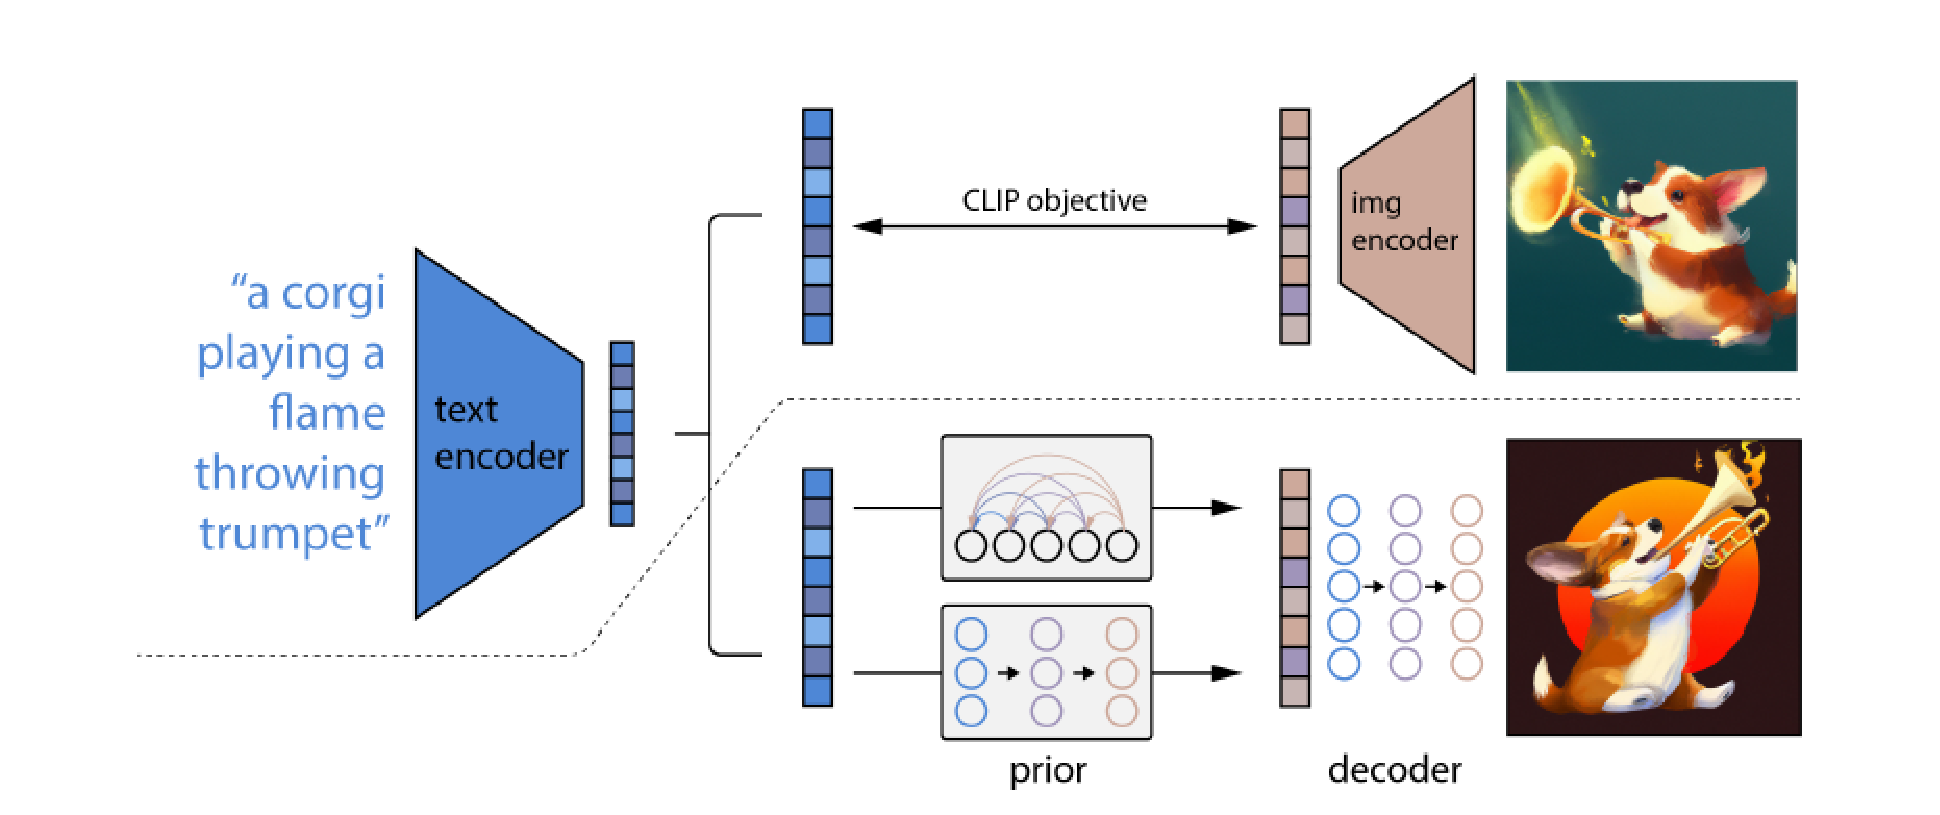
\includegraphics[width=0.7\textwidth]{dalle2.eps}
\caption{Prikaz DALL-E 2 modela iz ptičije perspektive}
\label{fig: dalle2slika}
\end{figure}

\end{frame}

\section{Kako bilo ko može da koristi AI za generisanje slika}	% 1 slajd

\begin{frame}[fragile]\frametitle{Kako bilo ko može da koristi AI za generisanje slika}
    \begin{itemize}
		\item Prednosti:
        \item[] Realizam, originalnost, konstanto napredovanje
        \item Mane:
        \item[] Nema emocija, ponavljanje, etički problemi
        \item Primeri:
		\item[] DALL-E 2
		\item[] Midjourney
	\end{itemize}
	
\end{frame}

\begin{frame}[fragile]\frametitle{Kako bilo ko može da koristi AI za generisanje slika}
	
\begin{figure}[htp]
\centering
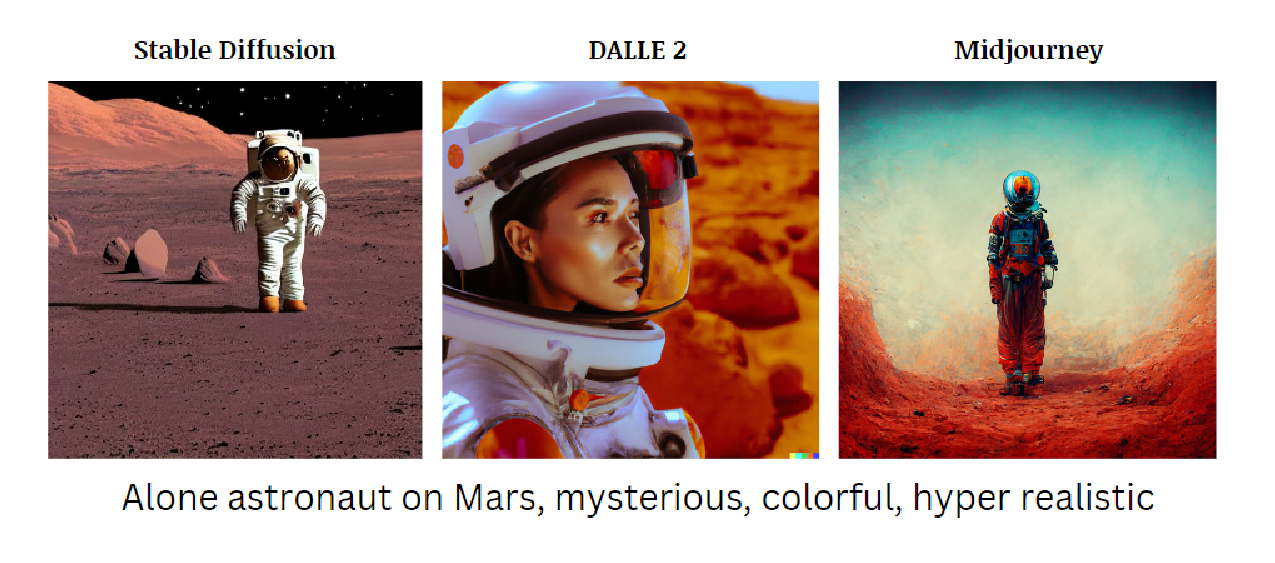
\includegraphics[width=1\textwidth]{astronaut.eps}
\caption{Poređenje ova tri AI generatora}
\label{fig: Astronaut}
\end{figure}
	
\end{frame}


\section{Etički problemi sa veštačko inteligentnim generatorima slika} % 1 slajd
\subsection{Autorska prava}

\begin{frame}[fragile]\frametitle{Etički problemi sa veštačko inteligentnim generatorima slika}
	
	\begin{itemize}
		\item Oponašavanje štetnih stereotipa
        \item[]  - Korigovanje prompt-ova (dodavanje reči)
        \item Problemi:
        \item[] - Kreiranje lažnih informacija, strah od lažnih dokaza
        \item Problem autorskih prava:
		\item[] - Ko polaže autorska prava nad generisanim sadržajem?
		\item[] - Komercijalna ili lična upotreba?
		\item[] - Uticaj na kreativnu industriju
	\end{itemize}	
	
\end{frame}

\section{Zaključak} % 1 slajd

\begin{frame}[fragile]\frametitle{Zaključak}
	
\end{frame}

\end{document}
